\documentclass[]{article}
\newcommand{\FileDepth}{../..}
\usepackage[a4paper, total={15cm,23cm}]{geometry}
\usepackage[T1]{fontenc}
\usepackage{textcomp}%Not strictly necessary, but gives \textmu command for "micro."
\usepackage{fancyhdr}
\usepackage{amsmath}
\usepackage{amssymb}
\usepackage{graphicx}
\usepackage{xcolor}
\usepackage{tikz}
\usetikzlibrary{calc}
%opening
\newcommand{\SecType}{X}
\newcommand{\Week}{X}
\title{Interpreting a Potential Energy Graph}
\author{Benjamin Bauml}
\date{Spring 2024}
\pagestyle{fancy}
\rhead{PH 221}
\chead{Spring 2024}
\lhead{Week \Week}

% For Assignment, leave Purpose as 1. For Worksheet, set to 2. For Student Solution, set to 3. For Teacher Solution, set to 4.
% If you want keep the pieces from being called manually, set DefOnly to 0.
\newcommand{\Purpose}{4}
\newcommand{\DefOnly}{1}

% Version 2024-04-27
% Changes
% 2024-02-21 Added xstring package to enable smooth implementation of new \ModePage command.
% 2024-04-27 Set up to split activities and formatting aspects into separate files. Removed dependence on xcomment. Added an automatic counter to number the activities in a problem set.
% 2024-05-19 Revised old format for \TeachingTips command, which did not support \DefOnly.
\usepackage{tcolorbox}
\usepackage{xstring}
% You will want the following four lines in your document (the last two uncommented):
% For Assignment, leave Purpose as 1. For Worksheet, set to 2. For Student Solution, set to 3. For Teacher Solution, set to 4.
% If you want keep the pieces from being called manually, set DefOnly to 0.
%\newcommand{\Purpose}{4}
%\newcommand{\DefOnly}{1}
\newcommand{\Exclusion}{0}
\newcommand{\PageTurn}{0}
\newcommand{\GrayProb}{0}
\newcommand{\Tipsy}{0}

% Assignment
\if\Purpose1
\renewcommand{\Exclusion}{1}
\fi
% Worksheet
\if\Purpose2
\renewcommand{\Exclusion}{1}
\renewcommand{\PageTurn}{1}
\fi
% Student Solution
\if\Purpose3
\renewcommand{\PageTurn}{1}
\renewcommand{\GrayProb}{1}
\fi
% Teaching Copy
\if\Purpose4
\renewcommand{\PageTurn}{1}
\renewcommand{\GrayProb}{1}
\renewcommand{\Tipsy}{1}
\fi

\def \NewQ {0}
\def \PForce {0}
\newcommand{\MaybePage}[1]{
	\def \PForce {#1}
	\if\PForce1
	\newpage
	\else
	\if\NewQ0
	\gdef \NewQ {\PageTurn}
	\else
	\newpage
	\fi
	\fi
}

\newcommand{\ModePage}[1]{
	\IfSubStr{#1}{\Purpose}{\newpage}{}
}

\newcounter{ActNumber}
\setcounter{ActNumber}{0}

\newcommand{\Problem}[4][0]{%The first argument is optional, and if it is set to 1, the \newpage will be forced. The second argument is the name of the activity, the third is the command the activity is stored as, and the fourth is the actual problem statement.
\newcommand{#3}{
\MaybePage{#1}
\addtocounter{ActNumber}{1}
\section*{\SecType\Week-\theActNumber: #2}
\if\GrayProb1
\begin{tcolorbox}[colback=lightgray,colframe=lightgray,sharp corners,boxsep=1pt,left=0pt,right=0pt,top=0pt,bottom=0pt,after skip=2pt]
\else
\begin{tcolorbox}[colback=white,colframe=white,sharp corners,boxsep=1pt,left=0pt,right=0pt,top=0pt,bottom=0pt,after skip=2pt]
\fi
#4
\end{tcolorbox}\noindent
}
\if\DefOnly0
\else
#3
\fi
}
	
\newcommand{\ProblemSub}[3][0]{%The first argument is optional, and if a string of numbers is entered into it, it will force a \newpage in any \Purpose that shows up in the string. For example, "13" would lead to the newpage being forced in modes 1 and 3. The second is the command the activity is stored as, and the third is the actual problem statement.
\newcommand{#2}{
\ModePage{#1}
\if\GrayProb1
\begin{tcolorbox}[colback=lightgray,colframe=lightgray,sharp corners,boxsep=1pt,left=0pt,right=0pt,top=0pt,bottom=0pt,after skip=2pt]
\else
\begin{tcolorbox}[colback=white,colframe=white,sharp corners,boxsep=1pt,left=0pt,right=0pt,top=0pt,bottom=0pt,after skip=2pt]
\fi
#3
\end{tcolorbox}\noindent
}
\if\DefOnly0
\else
#2
\fi
}
		
\newcommand{\Solution}[2]{%The first argument is the command the solution is stored as, and the second is the actual solution.
\newcommand{#1}{
\if\Exclusion0
#2
\fi
}
\if\DefOnly0
\else
#1
\fi
}
		
\newcommand{\ProblemFig}[2]{%The first argument is the command the figure is stored as, and the second is the actual figure.
\newcommand{#1}{
\begin{figure}[h]
#2
\end{figure}
}
\if\DefOnly0
\else
#1
\fi
}

\newcommand{\TeachingTips}[2]{%The first argument is the command the tip is stored as, and the second is the actual tip.
\newcommand{#1}{
\if\Tipsy1
\begin{tcolorbox}[colback=lightgray,colframe=black]
#2
\end{tcolorbox}
\fi
}
\if\DefOnly0
\else
#1
\fi
}

\begin{document}
\maketitle
\begin{center}
	This material is borrowed/adapted from Chapter 10 of the \textit{Student Workbook} for \textit{Physics for Scientists and Engineers}.
\end{center}

\Problem{Interpreting a Potential Energy Graph}{\InterPotEG}{
A particle with the potential energy shown in the graph is moving to the right at $ x = 0 $ m with total energy $ E $.
}
\ProblemFig{\InterPotEGFig}{
\centering
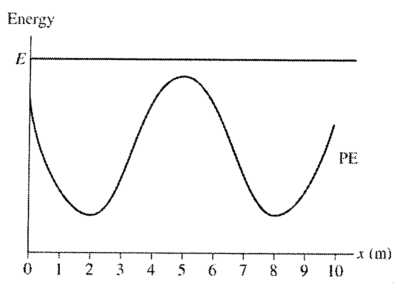
\includegraphics{\FileDepth/Activities/Interpreting_a_Potential_Energy_Graph/PE_Graph_to_Interpret.pdf}
}
\ProblemSub{\InterPotEGA}{
(a) At what value or values of $ x $ is the particle's speed a maximum?
}
\Solution{\InterPotEGASol}{

At 2 m and 8 m, where the potential energy is smallest.
}
\ProblemSub{\InterPotEGB}{
(b) At what value or values of $ x $ is the particle's speed a minimum?
}
\Solution{\InterPotEGBSol}{

At 5 m, where the potential energy is largest.
}
\ProblemSub{\InterPotEGC}{
(c) At what value or values of $ x $ is the potential energy a maximum?
}
\Solution{\InterPotEGCSol}{

At 5 m.
}
\ProblemSub{\InterPotEGD}{
(d) Does this particle have a turning point in the range of $ x $ covered by the graph? If so, where?
}
\Solution{\InterPotEGDSol}{

There are no turning points, as the potential energy never crosses the total energy line.
}
\ProblemSub{\InterPotEGE}{
(e) In which intervals of $ x $ is the force on the particle to the right?
}
\Solution{\InterPotEGESol}{

Since $ F_{x} = -\frac{dU}{dx} $ (negative of slope), we know that the force is to the right ($ F_{x} $ is positive) from 0 m to 2 m and from 5 m to 8 m.
}
\ProblemSub{\InterPotEGF}{
(f) In which intervals of $ x $ is the force on the particle to the left?
}
\Solution{\InterPotEGFSol}{

The force is to the left ($ F_{x} $ is negative) from 2 m to 5 m and from 8 m to 10 m.
}
\ProblemSub{\InterPotEGG}{
(g) At what value or values of $ x $ is the magnitude of the force a maximum?
}
\Solution{\InterPotEGGSol}{

When the slope of $ U $ versus $ x $ is steepest: $ x = 0 $ m, 3.5 m, 6.5 m, and 10 m.
}
\ProblemSub{\InterPotEGH}{
(h) At what value or values of $ x $ are positions of stable equilibrium?
}
\Solution{\InterPotEGHSol}{

Equilibrium occurs when $ F_{x} = 0 $ N. Stable equilibrium occurs when the force felt on either side of the point pushes the particle back toward the point. This happens at the minima of potential energy: $ x = 2 $ m and 8 m.
}
\ProblemSub{\InterPotEGI}{
(i) At what value or values of $ x $ are positions of unstable equilibrium?
}
\Solution{\InterPotEGISol}{

Unstable equilibrium occurs when the force felt on either side of the equilibrium point pushes the particle away from the point. This happens at the maximum of potential energy: $ x = 5 $ m.
}
\ProblemSub{\InterPotEGJ}{
(j) If the particle is released from rest at $ x = 0 $ m, will it reach $ x = 10 m $? Explain.
}
\Solution{\InterPotEGJSol}{

No. If released from rest, the particle's total energy is the initial potential energy and can never exceed this value. The particle will turn around at about $ x = 3.5 $ m.
}
\end{document}